%\part{First-order Numerical Methods}
\chapter{Numerical Experiments}\label{chap:chapter_5}
In Chapter~\ref{chap:chapter_3}, we developed the Lax--Friedrichs and Godunov schemes, including a complete algorithm for implementing the Lax--Friedrichs scheme \eqref{eq:Lax-F numerical flux}. In Chapter~\ref{chap:chapter_4}, we provided the stability analysis of \eqref{eq:generic_H_N} and concluded that the method is asymptotically compatible. In the present chapter, we first present numerical experiments in Section~\ref{sec:Comparison_left_Normalized} demonstrating that the choice of numerical quadrature weights $w_k$ plays an essential role in the asymptotic compatibility of the numerical method \eqref{eq:generic_H_N}. In Section~\ref{sec:Convergence_analysis}, we then provide numerical evidence for the convergence of the method.

\section{Comparison of Left endpoint  and Normalized Left endpoint}\label{sec:Comparison_left_Normalized}
We start by comparing the quadrature weights obtained from the left endpoint  and the normalized left endpoint .
For the Riemann problem \eqref{eq: Riemann problem}, we choose $u_L = 0.6$ and $u_R = 0.1$ such that the problem becomes to solve
\begin{equation}\label{eq:sloving rarefaction}
    \begin{split}
        u_{t} + f(u)_{x} & = 0 \\
        u(x,0)           & =
        \begin{cases}
            0.6 & \text{if } x < 0  \\
            0.1 & \text{if } x > 0.
        \end{cases}
    \end{split}
\end{equation}
Since $u_L > u_R $ , $h$ in \eqref{eq:h} equals
\[
    \inf\{ g(u) \mid g \geq f \text{ and } g \text{ is concave on } [u_R, u_L] \},
\]
since $f$ is concave, $h$ equals $f$ itself. Thus, the entropy solution is given by
\begin{equation}\label{eq: u_L > u_R}
    u(x,t) =
    \begin{cases}
        0.6               & \text{for } x \leq -0.2t,           \\
        \dfrac{t - x}{2t} & \text{for } -0.2t \leq x \leq 0.8t, \\
        0.1               & \text{for } x \geq 0.8t.
    \end{cases}
\end{equation}


Let us now choose $u_L = 0.1$ and $u_R = 0.6$ such that the problem becomes to solve
\begin{equation}\label{eq:sloving shocks}
    \begin{split}
        u_{t} + f(u)_{x} & = 0 \\
        u(x,0)           & =
        \begin{cases}
            0.1 & \text{if } x < 0  \\
            0.6 & \text{if } x > 0.
        \end{cases}
    \end{split}
\end{equation}
Since $u_L < u_R $ , $h$ in \eqref{eq:h} equals
\[
    \sup\{ g(u) \mid g \leq f \text{ and } g \text{ is convex on } [u_L, u_R] \},
\]
since $f$ is concave, $h$ must equal a linear function. This leads us to a solution that consists of $u_L$ and $u_R$, separated by a single shock with its speed $s$ given by the Rankine--Hugoniot condition such that
\begin{align*}
    s(t) & = \frac{f(u_R)- f(u_L)}{u_R- u_L}          \\
         & = \frac{0.6(1-0.6) - 0.1(1-0.1) }{0.6-0.1} \\
         & = 0.3.
\end{align*}
Hence, the solution is given by
\begin{equation}\label{eq: u_L < u_R}
    \begin{split}
        u(x,t) =
        \begin{cases}
            0.1 & \text{if } x < 0.3t  \\
            0.6 & \text{if } x > 0.3t.
        \end{cases}
    \end{split}
\end{equation}
We mention now that in all numerical experiments we do in this thesis, we choose the computational domain $[x_L, x_R] = [-2, 2]$, the linear kernel $\omega^{\epsilon}(y) = \frac{2(\epsilon-y)}{\epsilon^2}$  and the numerical viscosity $\alpha = 2$. So, we plot the rarefaction solution $u$ given by \eqref{eq: u_L > u_R} at final time $ T = 1$ together with both the local and nonlocal numerical approximations.

\subsection*{Numerical Experiment 1a}
We begin by implementing the Lax--Friedrichs type scheme \eqref{eq:Lax-F numerical flux} for $\epsilon = 0.1$ and $\Delta x = 0.02$

\begin{figure}[H]
    \centering
    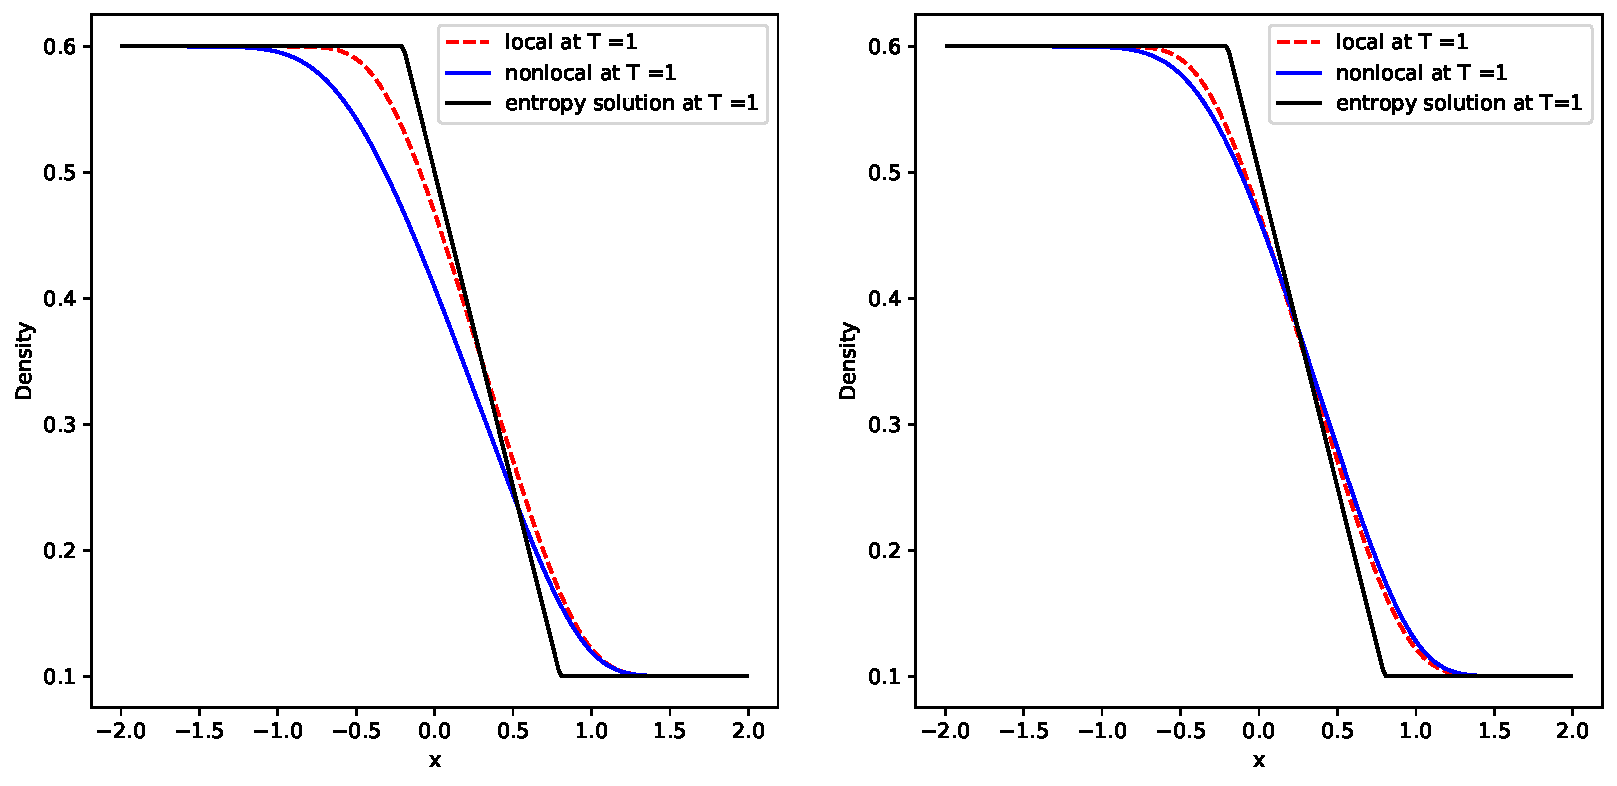
\includegraphics[width=\textwidth]{exp_1a.pdf}
    \caption{Numerical solutions and entropy solution at T = $1$ corresponding to the left endpoint numerical quadrature weights \eqref{eq:left_endpoint-quadrature} (left) and the normalized left endpoint numerical quadrature weights \eqref{eq:normalized_left_endpoint_quadrature}(right).}
    \label{fig:exp_1a}
\end{figure}
As shown in Figure~\ref{fig:exp_1a}, the choice of numerical quadrature weights does not lead to a significant difference between the numerical solutions and the entropy solution of the local model \eqref{eq:local model}. Nevertheless, a low level of accuracy remains at the shocks, where the numerical solutions deviate noticeably from the entropy solution. We aim to achieve convergence of the numerical solutions to the entropy solution as $\Delta x$ and $\epsilon$ tend to zero simultaneously.

\subsection*{Numerical Experiment 1b}
Next we choose $\epsilon = 0.01$ and $\Delta x = 0.005$

\begin{figure}[H]
    \centering
    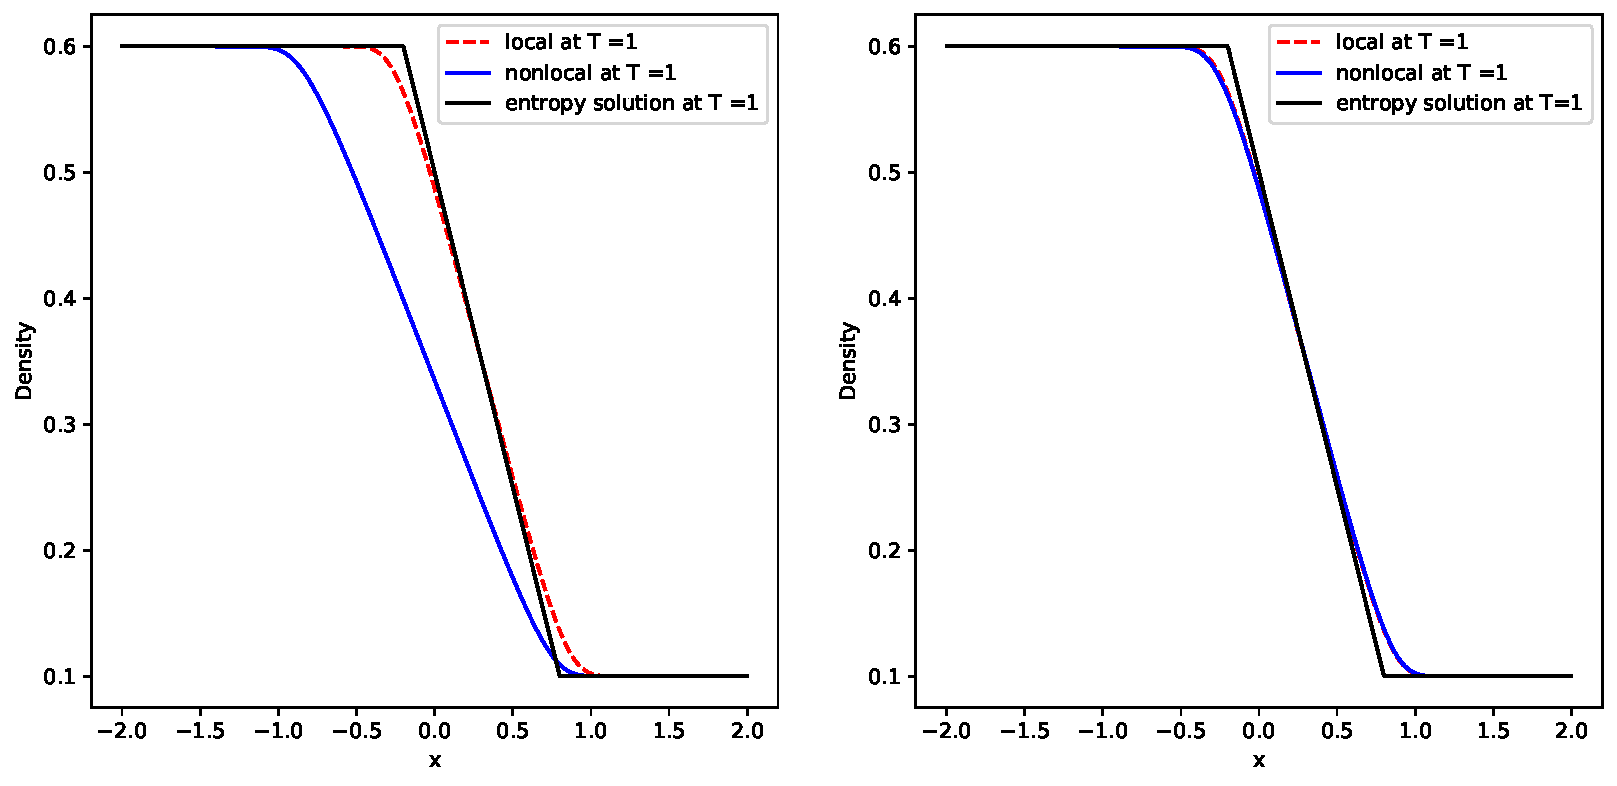
\includegraphics[width=\textwidth]{exp_1b.pdf}
    \caption{Numerical solutions and entropy solution at T = $1$ corresponding to the left endpoint numerical quadrature weights \eqref{eq:left_endpoint-quadrature} (left) and the normalized left endpoint numerical quadrature weights \eqref{eq:normalized_left_endpoint_quadrature} (right).}
    \label{fig:exp_1b}
\end{figure}
As observed in Figure~\ref{fig:exp_1b}, contrary to our expectations, the left endpoint numerical quadrature weights cause the numerical solution of the nonlocal model to deviate further from both the numerical solution and the entropy solution of the local model. In contrast, the normalized left endpoint quadrature weights lead to improved accuracy and better alignment between the numerical solutions and the entropy solution.

\subsection*{Numerical Experiment 1c}
Finally we take $\epsilon = 0.001$ and $\Delta x = 0.001$.
\begin{figure}[H]
    \centering
    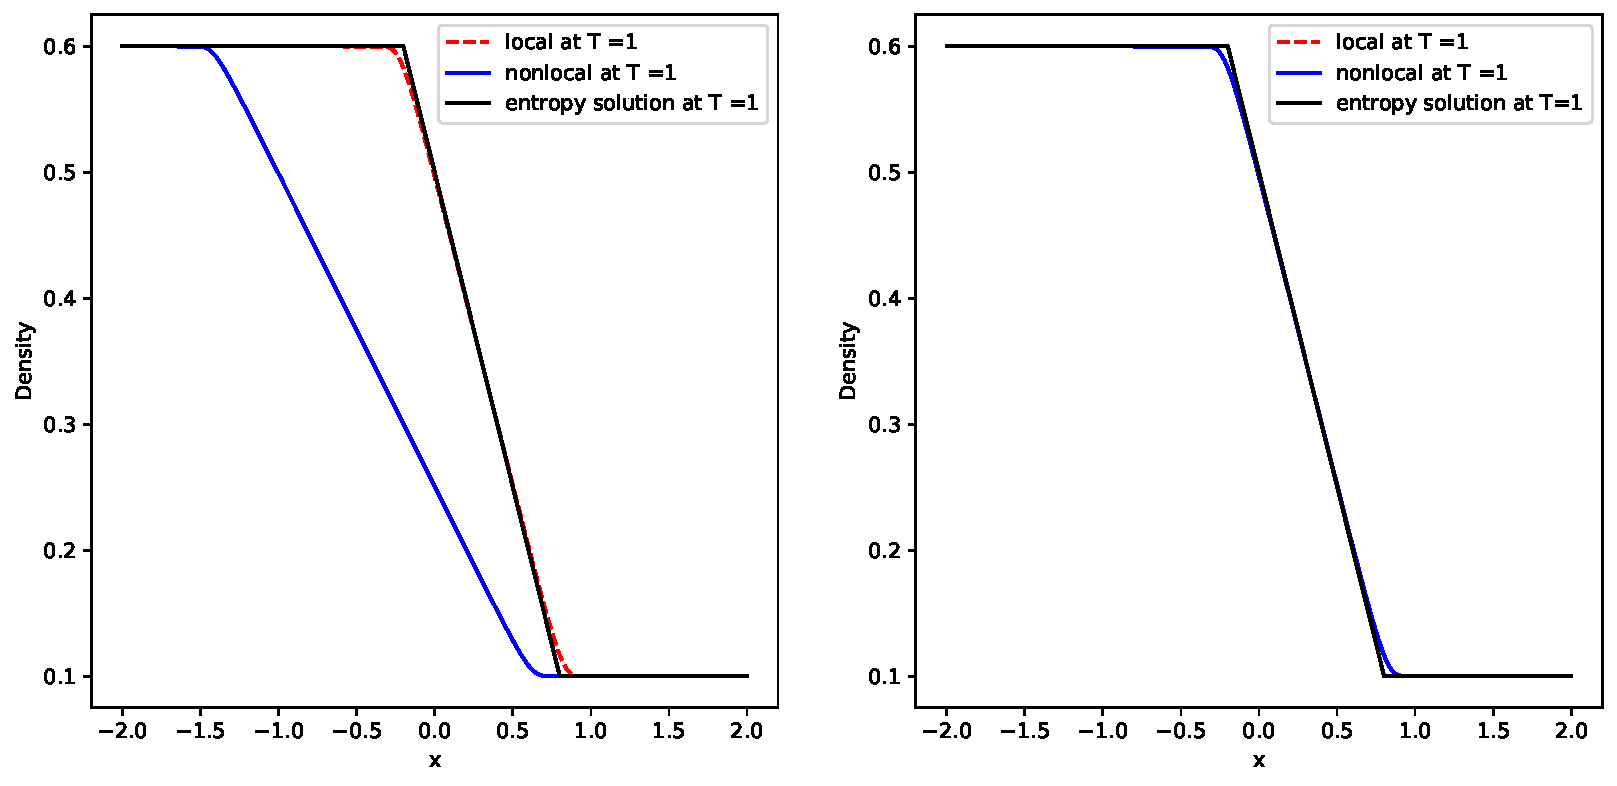
\includegraphics[width=\textwidth]{exp_1c.pdf}
    \caption{Numerical solutions and entropy solution at T = $1$ corresponding to the left endpoint numerical quadrature weights \eqref{eq:left_endpoint-quadrature} (left) and the normalized left endpoint numerical quadrature weights \eqref{eq:normalized_left_endpoint_quadrature} (right).}
    \label{fig:exp_1c}
\end{figure}
We observe in Figure~\ref{fig:exp_1c} that the numerical solution of the nonlocal model obtained using the left endpoint numerical quadrature weights completely fails. By contrast, significantly better accuracy is observed when using the normalized left endpoint numerical quadrature weights.
\subsection*{Summary}
The numerical experiments above demonstrate that, as $\Delta x$ and $\epsilon$ tend to zero simultaneously, while the Lax--Friedrichs type scheme based on the left endpoint quadrature weights becomes increasingly inaccurate, the normalized left endpoint quadrature weights consistently maintain stability and improved alignment with the entropy solution. The reason for this lies on the normalization condition, i.e, the sum of the numerical quadrature $w_k$ equals $1$. The above results provide evidence that the choice of numerical quadrature weights plays a crucial role in ensuring the asymptotic compatibility of the numerical method \eqref{eq:generic_H_N}.

\section{Numerical Convergence Analysis}\label{sec:Convergence_analysis}
The numerical experiments above indicate that the method \eqref{eq:generic_H_N} is consistent and stable when using the normalized left endpoint quadrature weights. We continue the numerical experiment to determine the convergence and order of convergence, and see if the Godunov numerical scheme\eqref{eq:God_F} is more accurate than the Lax--Friedrichs scheme \eqref{eq:Lax-F numerical flux}.
We are interested in presenting numerical experiments on whether:
\begin{itemize}
    \item $\rho^{\epsilon, \Delta x} \rightarrow u$ as both $\Delta x \rightarrow 0$ and $\epsilon \rightarrow 0$ simultaneously.
    \item $\rho^{\epsilon, \Delta x} \rightarrow \rho^{\epsilon}$ for fixed $\epsilon$ as $\Delta x \rightarrow 0$.
\end{itemize}

Considering the computed reference and numerical solutions as piecewise constant functions on each cell of size $\Delta x$, we measure the global error
\[
    e = U^{\mathrm{ref}} - U^{\mathrm{num}}
\]
using the $L^{1}$ norm:
\begin{align*}
    \| e \|_{L^{1}} = \Delta x \sum_{j=0}^{K-1} |e^j|.
\end{align*}
Here, $U^{\mathrm{ref}}$ and $U^{\mathrm{num}}$ denote the reference solution and the numerical solution, respectively. We aim to obtain
\[
    \| e \|_{L^{1}} \rightarrow 0
\]
as the parameters tend to zero.

\subsection{Numerical Convergence to the Local Model}
%\textcolor{red}{Rarefaction solution}
We will present the numerical experiments for $\rho^{\epsilon, \Delta x} \rightarrow u $ as both $\Delta x \rightarrow 0$ and $\epsilon \rightarrow 0$ simultaneously. In addition to the initial data \eqref{eq:sloving rarefaction} and \eqref{eq:sloving shocks}, we also consider the smooth initial data
\begin{equation}\label{eq:smooth}
    u(x,0) = 0.5 + 0.3\cos{\frac{\pi x}{2}}.
\end{equation}

We remember that, as described in Chapter~\ref{chap:chapter_2}, we have a formula for solving Riemann problems of the local model. Hence for the Riemann initial data \eqref{eq:sloving rarefaction} and \eqref{eq:sloving shocks} we take the corresponding reference solution $u$ to be the exact entropy solution given by \eqref{eq: u_L > u_R} and \eqref{eq: u_L < u_R}, respectively. For the smooth initial data \eqref{eq:smooth}, we compute the corresponding reference solution $u$ numerically on a fine grid for $\Delta x = \frac{4}{4096}$. With the relation $\epsilon = 3\Delta x$, we let both $\Delta x \rightarrow 0$ and \(\epsilon \to 0\) simultaneously, although $\Delta x = \frac{1}{2^{4+m}}$ for $m = 0,1,2,3, 4, 5,6$, and compute the $L^{1}$ errors and order of convergence.

Focusing on the initial data given in \eqref{eq:sloving rarefaction}, we plot the $L^{1}$ errors against the number of cells to compare the efficiency of the Godunov and Lax--Friedrichs scheme. We also present the observed order of convergence in Table~\ref{tab:table_1}
\begin{figure}[H]
    \centering
    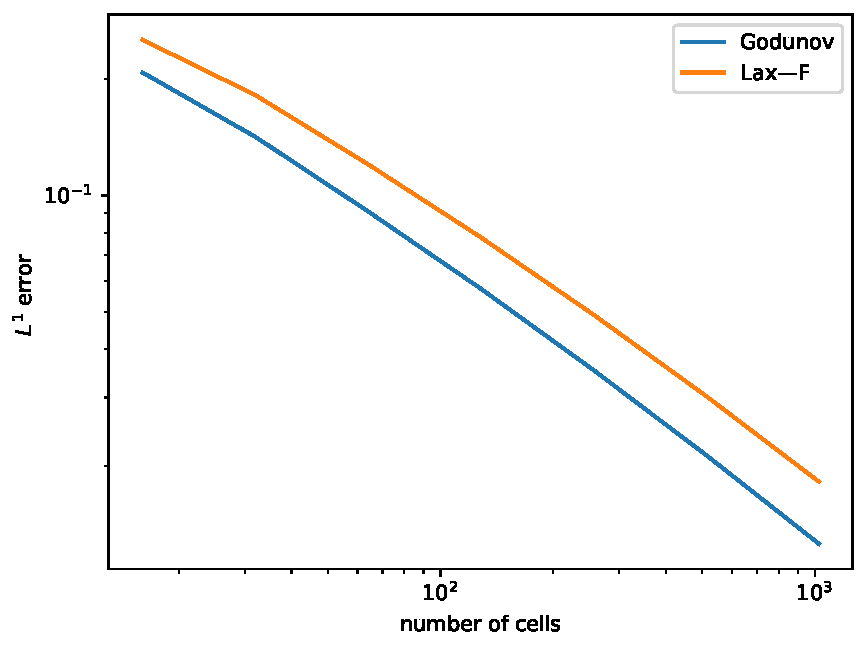
\includegraphics[width=0.7\textwidth]{Conver_local.pdf}
    \caption{$L^1$ error vs. number of cells}
    \label{fig:Conver_local_1}
\end{figure}
Figure~\ref{fig:Conver_local_1} indicates that the $L^{1}$-error for both Godunov and Lax--Friedrichs scheme tends to zero as the number of cells increases.
In other words, both the schemes converge to the unique entropy solution $u$ of the local model \eqref{eq:local model} as both \(\Delta x \to 0\) and \(\epsilon \to 0\) simultaneously. We observe as well that the Godunov scheme converges faster than Lax--Friedrichs scheme.
A natural question is: how fast do the schemes converge?
To answer this, we study the order of convergence $r$ for both schemes.

We assume that the $L^{1}$ error on a mesh of size $\Delta x_i$ can be written as
\begin{align*}
    E_i = C(\Delta x_i)^r,
\end{align*}
for some constant $C>0$.
If we have the error at two consecutive refinement levels $(E_{i-1},E_i)$, then we have
\begin{align*}
    \frac{E_{i-1}}{E_i}
    =\left(\frac{\Delta x_{i-1}}{\Delta x_i}\right)^{r}.
\end{align*}
Taking logarithms on both sides gives the standard expression for the order of convergence
\begin{align*}
    r =
    \frac{\log(E_{i-1}) - \log(E_i)}
    {\log(\Delta x_{i-1}) - \log(\Delta x_i)}.
\end{align*}
The order of convergence tells us how fast does a scheme converge to the correct solution, the higher order is the faster convergence.

\begin{table}[H]
    \centering
    \begin{minipage}{0.45\textwidth}
        \centering
        \begin{tabular}{ |p{1.5cm}||p{2.2cm}| |p{1.5cm}| }
            \hline
            \textbf{Cells } & $L^{1}$-\textbf{errors}  & \textbf{OOC} \\
            \hline
            16              & $2.5205 \times 10^{-1}$  & --           \\
            32              & $1.8141 \times 10^{-1}$  & 0.4744       \\
            64              & $1.2020 \times 10^{-1}$  & 0.5938       \\
            128             & $7.7851 \times 10^{-2}$  & 0.6267       \\
            256             & $4.9129 \times 10^{-2}$  & 0.6641       \\
            512             & $3.0257 \times 10^{-2}$  & 0.6993       \\
            1024            & $1.8184 \times 10^{-2} $ & 0.7346       \\
            \hline
        \end{tabular}
        \caption*{(a) Lax--Friedrichs scheme}
    \end{minipage}
    \hfill
    \begin{minipage}{0.5\textwidth}
        \centering
        \begin{tabular}{ |p{1.5cm}||p{2.2cm}| |p{1.5cm}| }
            \hline
            \textbf{Cells } & $L^{1}$-\textbf{errors} & \textbf{OOC} \\
            \hline
            16              & $2.0744 \times 10^{-1}$ & --           \\
            32              & $1.4154 \times 10^{-1}$ & 0.5515       \\
            64              & $9.0816 \times 10^{-2}$ & 0.6402       \\
            128             & $5.7350 \times 10^{-2}$ & 0.6632       \\
            256             & $3.5334 \times 10^{-2}$ & 0.6987       \\
            512             & $2.1299 \times 10^{-2}$ & 0.7303       \\
            1024            & $1.2565 \times 10^{-2}$ & 0.7614       \\
            \hline
        \end{tabular}
        \caption*{(b) Godunov scheme}
    \end{minipage}

    \caption{$L^{1}$-errors and observed order of convergence obtained using the Lax--Friedrichs scheme and the Godunov scheme in solving the local model with the Riemann initial data \eqref{eq:sloving rarefaction}.}
    \label{tab:table_1}
\end{table}
Table \ref{tab:table_1} presents the quantitative results for the $L^{1}$-errors and the observed order of convergence $r$ for the
Riemann initial data \eqref{eq:sloving rarefaction}, where $u_L > u_R$. We observe that the $L^{1}$-errors produced by the Godunov scheme are consistently smaller than those obtained using the Lax--Friedrichs scheme. For both schemes, the observed order of convergence is at most $1$, indicating relatively slow convergence.

Let us now consider the Riemann initial data \eqref{eq:sloving shocks}, where $u_L < u_R$.
We obtain the corresponding quantitative results:
\begin{table}[H]
    \centering
    \begin{minipage}{0.45\textwidth}
        \centering
        \begin{tabular}{ |p{1.5cm}||p{2.2cm}| |p{1.5cm}| }
            \hline
            \textbf{Cells } & $L^{1}$-\textbf{errors} & \textbf{OOC} \\
            \hline
            16              & $2.3182 \times 10^{-1}$ & --           \\
            32              & $1.4869 \times 10^{-1}$ & 0.6407       \\
            64              & $8.8979 \times 10^{-2}$ & 0.7408       \\
            128             & $5.0150 \times 10^{-2}$ & 0.8272       \\
            256             & $2.6012 \times 10^{-2}$ & 0.9470       \\
            512             & $1.3128 \times 10^{-2}$ & 0.9866       \\
            1024            & $6.5769 \times 10^{-3}$ & 0.9971       \\
            \hline
        \end{tabular}
        \caption*{(a) Lax--Friedrichs scheme}
    \end{minipage}
    \hfill
    \begin{minipage}{0.5\textwidth}
        \centering
        \begin{tabular}{ |p{1.5cm}||p{2.2cm}| |p{1.5cm}| }
            \hline
            \textbf{Cells } & $L^{1}$-\textbf{errors} & \textbf{OOC} \\
            \hline
            16              & $1.2876 \times 10^{-1}$ & --           \\
            32              & $8.5352 \times 10^{-2}$ & 0.5932       \\
            64              & $4.9126 \times 10^{-2}$ & 0.7969       \\
            128             & $2.6836 \times 10^{-2}$ & 0.8723       \\
            256             & $1.3336 \times 10^{-2}$ & 1.0089       \\
            512             & $6.7539 \times 10^{-3}$ & 0.9815       \\
            1024            & $3.3509 \times 10^{-3}$ & 1.0112       \\
            \hline
        \end{tabular}
        \caption*{(b) Godunov scheme}
    \end{minipage}
    \caption{$L^{1}$-errors and observed order of convergence obtained using the the Lax--Friedrichs scheme and the Godunov scheme in solving the local model with the Riemann initial data \eqref{eq:sloving shocks}}
    \label{tab:table_2}
\end{table}
The observation in Table \ref{tab:table_2} indicates that the Godunov numerical scheme handles solutions with shocks effectively than The Lax--Friedrichs scheme. We also observe that for both schemes the order of convergence is $1$.

Finally we repeat the above experiments with the smooth initial data \eqref{eq:smooth}, and obtain the corresponding quantitative results
\begin{table}[H]
    \centering
    \begin{minipage}{0.45\textwidth}
        \centering
        \begin{tabular}{ |p{1.5cm}||p{2.2cm}| |p{1.5cm}| }
            \hline
            \textbf{Cells } & $L^{1}$-\textbf{errors} & \textbf{OOC} \\
            \hline
            16              & $4.4055 \times 10^{-1}$ & --           \\
            32              & $2.7531 \times 10^{-1}$ & 0.6783       \\
            64              & $1.6123 \times 10^{-1}$ & 0.7719       \\
            128             & $9.0595 \times 10^{-2}$ & 0.8316       \\
            256             & $4.9132 \times 10^{-2}$ & 0.8828       \\
            512             & $2.5445 \times 10^{-2}$ & 0.9493       \\
            1024            & $1.2221 \times 10^{-2}$ & 1.0580       \\
            \hline
        \end{tabular}
        \caption*{(a) Lax--Friedrichs scheme}
    \end{minipage}
    \hfill
    \begin{minipage}{0.5\textwidth}
        \centering
        \begin{tabular}{ |p{1.5cm}||p{2.2cm}| |p{1.5cm}| }
            \hline
            \textbf{Cells } & $L^{1}$-\textbf{errors}  & \textbf{OOC} \\
            \hline
            16              & $3.1431 \times 10^{-1}$  & --           \\
            32              & $1.8983 \times 10^{-1}$  & 0.7275       \\
            64              & $1.0959 \times 10^{-1}$  & 0.7926       \\
            128             & $6.1083 \times 10^{-2}$  & 0.8433       \\
            256             & $3.3016 \times 10^{-2}$  & 0.8876       \\
            512             & $1.7172 \times 10^{-2}$  & 0.9432       \\
            1024            & $ 8.4201 \times 10^{-3}$ & 1.0281       \\
            \hline
        \end{tabular}
        \caption*{(b) Godunov scheme}
    \end{minipage}

    \caption{$L^{1}$-errors and observed order of convergence obtained using the the Lax--Friedrichs scheme and the Godunov scheme in solving the local model with smooth initial data \eqref{eq:smooth}.}
    \label{tab:table_3}
\end{table}
\subsection*{Summary}
The experiments above provide evidence that the numerical schemes are asymptotically compatible, in the sense that they converge to the entropy solution of the local model \eqref{eq:local model} as both parameters $\Delta x$ and $\epsilon$ tend to zero simultaneously. Moreover, although the stability analysis in Chapter~\ref{chap:chapter_4} is established under the assumption that the initial data can not contain negative jumps, the numerical experiments indicate that the methods remain robust even for the initial data \eqref{eq:sloving rarefaction}, which contains a negative jump.

\subsection{Numerical Convergence to the Nonlocal Model}

For fixed $\epsilon$, through numerical experiments we aim to deduce $ \| e \Vert_{L^{1}}= \| \rho^{\epsilon} - \rho^{\epsilon, \Delta x}\Vert_{L^{1}} \rightarrow 0$ as $\Delta x \rightarrow 0$. We compute the reference solution $\rho^{\epsilon}$ numerically for $\Delta x = \frac{4}{4096}$ and $\epsilon = 0.1$. Holding $\epsilon = 0.1$ fixed and letting $\Delta x \rightarrow 0$, although $\Delta x = \frac{1}{2^{4+m}}$ for $m = 0,1,2,3, 4, 5, 6$, we compute the $L^{1}$ errors and order of convergence.

%\begin{figure}[H]
%\centering
%
\includegraphics[width=0.7\textwidth]{Conver_2l.pdf}
%\caption{$L^1$ error vs. number of cells}
%\label{fig:Conver_1}
%\end{figure}

\begin{table}[H]
    \centering
    \begin{minipage}{0.45\textwidth}
        \centering
        \begin{tabular}{ |p{1.5cm}||p{2.2cm}| |p{1.5cm}| }
            \hline
            \textbf{Cells } & $L^{1}$-\textbf{errors}  & \textbf{OOC} \\
            \hline
            16              & $1.8626 \times 10^{-1}$  & --           \\
            32              & $1.2159 \times 10^{-1}$  & 0.6154       \\
            64              & $7.4547 \times 10^{-2}$  & 0.7058       \\
            128             & $ 4.2751 \times 10^{-2}$ & 0.8022       \\
            256             & $2.3350 \times 10^{-2}$  & 0.8725       \\
            512             & $1.1829 \times 10^{-2}$  & 0.9811       \\
            1024            & $5.3589 \times 10^{-3}$  & 1.1423       \\
            \hline
        \end{tabular}
        \caption*{(a) Lax--Friedrichs scheme}
    \end{minipage}
    \hfill
    \begin{minipage}{0.5\textwidth}
        \centering
        \begin{tabular}{ |p{1.5cm}||p{2.2cm}| |p{1.5cm}| }
            \hline
            \textbf{Cells } & $L^{1}$-\textbf{errors}  & \textbf{OOC} \\
            \hline
            16              & $1.2667 \times 10^{-1}$  & --           \\
            32              & $ 7.3044 \times 10^{-2}$ & 0.7942       \\
            64              & $4.2832 \times 10^{-2}$  & 0.7701       \\
            128             & $2.3189 \times 10^{-2}$  & 0.8853       \\
            256             & $1.2184 \times 10^{-2}$  & 0.9285       \\
            512             & $5.9654 \times 10^{-3}$  & 1.0303       \\
            1024            & $ 2.6423 \times 10^{-3}$ & 1.1748       \\
            \hline
        \end{tabular}
        \caption*{(b) Godunov scheme}
    \end{minipage}

    \caption{$L^{1}$-errors and observed order of convergence obtained using the the Lax--Friedrichs scheme and the Godunov scheme in solving the nonlocal model with the Riemann initial data \eqref{eq:sloving rarefaction}.}
    \label{tab:table_4}
\end{table}

\begin{table}[H]
    \centering
    \begin{minipage}{0.45\textwidth}
        \centering
        \begin{tabular}{ |p{1.5cm}||p{2.2cm}| |p{1.5cm}| }
            \hline
            \textbf{Cells } & $L^{1}$-\textbf{errors} & \textbf{OOC} \\
            \hline
            16              & $2.0628 \times 10^{-1}$ & --           \\
            32              & $1.0767 \times 10^{-1}$ & 0.9380       \\
            64              & $7.1225 \times 10^{-2}$ & 0.5962       \\
            128             & $3.8519 \times 10^{-2}$ & 0.8868       \\
            256             & $2.0491 \times 10^{-2}$ & 0.9106       \\
            512             & $1.0478 \times 10^{-2}$ & 0.9676       \\
            1024            & $4.8977 \times 10^{-3}$ & 1.0972       \\
            \hline
        \end{tabular}
        \caption*{(a) Lax--Friedrichs scheme}
    \end{minipage}
    \hfill
    \begin{minipage}{0.5\textwidth}
        \centering
        \begin{tabular}{ |p{1.5cm}||p{2.2cm}| |p{1.5cm}| }
            \hline
            \textbf{Cells } & $L^{1}$-\textbf{errors} & \textbf{OOC} \\
            \hline
            16              & $1.0844 \times 10^{-1}$ & --           \\
            32              & $4.4663 \times 10^{-2}$ & 1.2798       \\
            64              & $3.3717 \times 10^{-2}$ & 0.4056       \\
            128             & $1.6571 \times 10^{-2}$ & 1.0248       \\
            256             & $8.2085 \times 10^{-3}$ & 1.0134       \\
            512             & $3.9258 \times 10^{-3}$ & 1.0641       \\
            1024            & $1.7225 \times 10^{-3}$ & 1.1885       \\
            \hline
        \end{tabular}
        \caption*{(b) Godunov scheme}
    \end{minipage}

    \caption{$L^{1}$-errors and observed order of convergence obtained using the the Lax--Friedrichs scheme and the Godunov scheme in solving the nonlocal model with the Riemann initial data \eqref{eq:sloving shocks}}
    \label{tab:table_5}
\end{table}


\begin{table}[H]
    \centering
    \begin{minipage}{0.45\textwidth}
        \centering
        \begin{tabular}{ |p{1.5cm}||p{2.2cm}| |p{1.5cm}| }
            \hline
            \textbf{Cells } & $L^{1}$-\textbf{errors}  & \textbf{OOC} \\
            \hline
            16              & $3.3092 \times 10^{-1}$  & --           \\
            32              & $1.8065 \times 10^{-1} $ & 0.8733       \\
            64              & $9.9861 \times 10^{-2} $ & 0.8552       \\
            128             & $5.2189 \times 10^{-2}$  & 0.9362       \\
            256             & $2.6458 \times 10^{-2}$  & 0.9801       \\
            512             & $1.2647 \times 10^{-2}$  & 1.0649       \\
            1024            & $ 5.5133 \times 10^{-3}$ & 1.1978       \\
            \hline
        \end{tabular}
        \caption*{(a) Lax--Friedrichs scheme}
    \end{minipage}
    \hfill
    \begin{minipage}{0.5\textwidth}
        \centering
        \begin{tabular}{ |p{1.5cm}||p{2.2cm}| |p{1.5cm}| }
            \hline
            \textbf{Cells } & $L^{1}$-\textbf{errors} & \textbf{OOC} \\
            \hline
            16              & $1.8322 \times 10^{-1}$ & --           \\
            32              & $8.6063 \times 10^{-2}$ & 1.0901       \\
            64              & $4.5197 \times 10^{-2}$ & 0.9291       \\
            128             & $2.2487 \times 10^{-2}$ & 1.0071       \\
            256             & $1.1061 \times 10^{-2}$ & 1.0237       \\
            512             & $5.1421 \times 10^{-3}$ & 1.1050       \\
            1024            & $2.2161 \times 10^{-3}$ & 1.2143       \\
            \hline
        \end{tabular}
        \caption*{(b) Godunov scheme}
    \end{minipage}

    \caption{$L^{1}$-errors and observed order of convergence obtained using the the Lax--Friedrichs scheme and the Godunov scheme in solving the nonlocal model with the smooth initial data \eqref{eq:smooth}.}
    \label{tab:table_6}
\end{table}
\subsection*{Summary}
The quantitative results above indicate that for fixed $\epsilon$, $\rho^{\epsilon, \Delta x} \rightarrow \rho^{\epsilon} $ as $\Delta x \rightarrow 0$. In addition, the Godunov scheme is more efficient than the Lax--Friedrichs scheme. In addition, based on our numerical experiments, the order of the developed numerical schemes is at most $1$. So, in the next chapter we will develop a second-oder numerical scheme.

